 \section{Introduction}
\label{sec:Introduction}

A modern high-performance, cache-coherent, distributed-memory hardware system
is inherently complex. Such a system implements memory models like sequential
consistency (SC)~\cite{lamport1979make}, Total Store Order (TSO), and Relaxed
Memory Order (RMO)~\cite{weaver1994sparc}, each of which characterizes how
loads and stores may be issued by a processor and how the shared-memory
component responds to these requests.  These systems by their nature are highly
concurrent and nondeterministic.  The goal of this work is to provide a
framework for full verification of such complex hardware systems.  

Modularity has long been understood as a key property for effective design and
verification of such complex systems. For the designer, it allows a separation
of concerns, increasing robustness by allowing the behavior encapsulated by a
modular boundary to be realized by multiple implementations, any of which may
be dropped into the system safely. It also allows a greater parallelization of
human design effort, improving development time. Similarly, verification is
simplified, as modular interface agreements provide a natural lemma structure.
They lead us towards a decomposition of the whole-system verification task
into lemmas about subsystems, which can be composed in a black-box manner to
produce full-system theorems.

In this paper, we introduce \emph{a new approach to modular, deductive
verification of hardware designs} at the highest level of rigor, backed by
proofs using the Coq proof assistant.  As a challenging case study, we focus on
\emph{verifying that a particular infinite family of multicore, shared-memory
systems implements sequential consistency}.  The proof is parametrized over an
unknown number of processors connected to an arbitrary memory hierarchy with an
unknown number of caches in an unknown number of layers (e.g., L1, L2).  In our
design, processors and memory systems both independently employ intricate
optimizations that exploit opportunities for parallelism.  We are able to prove
that each of those two main components still provides strong enough guarantees
to support SC, and then we compose those theorems into a result for the full
system.  Either component may be optimized further without requiring any
changes to the implementation, specification, or proof of the other.

To structure our hardware verification framework, we use \emph{labeled
transition systems (LTSes)}, a well-studied approach in the world of
concurrent software modeling.  As our unified notion of specification and
proof, we adopt \emph{trace refinement}, which captures when one concurrent
system can only produce observable IO behaviors that another system could also
produce.  Each of our realistic hardware components is associated with a
simpler ``reference implementation'' that serves as a specification, and we
prove that each realistic component refines its spec.  Thereafter, it is sound
to use the simpler spec component in reasoning about the behavior of the
system.

Each key component of our case-study system has a simple spec: the ideal memory
responds instantly and atomically to each load or store request, and the ideal
processor executes instructions in order with no speculation.  The optimized
implementation of each is much more complicated: the cache-hierarchy memory
system potentially allows every cache to be busy simultaneously computing and
sending messages, and the optimized speculative processor sends multiple load
requests to the memory concurrently, without waiting for responses first.  The meat
of the verification is in showing that each optimized component refines its
simpler counterpart.  After each such proof, we may in effect substitute the
optimized version for the simple version in a black-box way within a design,
with a full guarantee of soundness.

LTSes as hardware descriptions are an established
idea \cite{HoeArvind:TRSSynthesis1, Hoe:TCAD}, and there are compilers that
convert LTSes into efficient hardware.  Our work is based on the Bluespec
language \cite{BSV:LangRef, Bluespec:TFRG}, which served as the model for the
formalism of this paper.  Bluespec models hardware components as atomic rules
of a transition system over state elements, and there is a commercial compiler
to synthesize such codes into register-transfer-level circuits (i.e., Verilog code) with
competitive performance.  Our cache-coherent memory system is directly
transliterated from a Bluespec
implementation \cite{DNA:CoherenceImplementation} used to implement a
cycle-accurate simulator for a cache-coherent multiprocessor PowerPC system \cite{Khan:PowerPc}. The hardware synthesized
from that implementation is rather efficient: an 8-core system with a 2-level
cache hierarchy can run 55 million instructions per second on the BEE FPGA
board \cite{bee2}.

Figure \ref{both} gives an example of an LTS inference rule
transliterated directly from an actual Bluespec rule used in the PowerPC
system.  Its meaning will become clear in Section \ref{sec:cc};
for now we just note that, while Bluespec rules employ Boolean \emph{guard}
conditions paired with sequences of imperative \emph{actions} to update state,
our (equivalent) formalization follows a natural-deduction inference-rule style,
where we explain a state transition as a relation between two tuples of state
elements, using rule premises where Bluespec uses guards.  The high-level point
is that the natural-deduction style is a semantically trivial rephrasing of the
Bluespec notation, which has been demonstrated as practical for synthesizing
realistic, high-performance hardware.  Inference rules like the one in
Figure \ref{both} fit naturally with the inductive-definition mechanisms of
proof systems like Coq, providing an effective starting point for formal
verification of hardware designs.

The main contributions of this paper are:
\vspace{-.3cm}
\begin{itemize} 
\item Identification of an interface between the processor and the memory
components of a multiprocessor system that enables modular implementation and
verification.

\item A general \emph{modular verification methodology} applicable to hardware
algorithms, based on \emph{labeled transition systems}.  We are able to verify
the several components of a modern processor against general formal interfaces,
enabling mixing and matching of different realizations of each interface,
without doing any new proofs that peek beneath abstraction boundaries.

\item The \emph{first machine-checked proof} of an implementation of sequential
consistency involving speculative processors and cache-coherent distributed
memory.

\item The \emph{first machine-checked proof} of an invalidation-based
cache-coherence protocol for distributed memories comprised of arbitrary cache
hierarchies. We believe such a memory is also the correct abstraction for
implementing relaxed memory models.
\end{itemize}

Overall, our agenda is to import, to the architecture domain, good ideas from
the worlds of programming-language semantics and formal software verification.
Wearing our architecture hats, we have found some of the proof insights to yield
surprising wisdom about hardware design, and we are optimistic that the
programming-languages perspective on modular verification will pay even more
dividends for reliable hardware design and verification.

\paragraph{Paper Organization:} We begin with a discussion of related work in
Section~\ref{relatedWork}. In Section~\ref{sec:lts} we introduce our flavor of
the labeled transition systems formalism, including a definition of trace
refinement. In Section~\ref{sec:store-atomicity}, we show a generic
decomposition of any multiprocessor system independently of the memory model
that it implements, and we discuss the store-atomicity property of the memory
subcomponent. In Section~\ref{sec:sc} we give a simple formal model of
sequential consistency.  The following sections refine the two main
subcomponents of our multiprocessor system.  Section~\ref{sec:ooo} discusses
definition and verification of a speculative processor model, and
Section~\ref{sec:cc} defines and proves our hierarchical cache-coherence
protocol.  Finally, in Section~\ref{sec:finalresult} we show the whole-system
modular proof of our complex system, and we end with some conclusions in
Section~\ref{sec:conclusion}.

\begin{figure}[t]
\centering
\begin{boxedminipage}{\columnwidth}
\small
\noindent \textbf{rule} $(c.\parent == p \; \mathit{\&\&} \; c.\s[a] < x \; \mathit{\&\&} \; c.\wt[a]== \textrm{None});$

\hspace{1cm} $\ch[c][p][\req].\enq(a,c.\s[a],x); c.\wt[a] \Leftarrow x;$

\textbf{endrule}
\end{boxedminipage}
\begin{boxedminipage}{\columnwidth}
\small
\inference[]
{\parent(c,p) & \s(c,a) < x & \wt(c,a) = \epsilon}
{\hspace{-.4cm}\ioxe{$M_c$}
{\hspace{-.2cm}\dt, \ch, \s,\hspace{-.2cm}\\
\hspace{-.2cm}\dst, \wt, \dwt,\hspace{-.2cm}\\
\hspace{-.2cm}\inp, \outp\hspace{-.2cm}}
{\hspace{-.2cm}\dt, \ch[ (c, p, \req) \coloneqq(a, \s(c, a),x)\hspace{-.2cm}\\
\;\;\;\;\;\;\uplus \ch(c,p,\req)], \s, \dst,\hspace{-.2cm}\\
\hspace{-.2cm}\wt[(c,a)\coloneqq x], \dwt,\inp, \outp\hspace{-.2cm}}{}\hspace{-.4cm}}
\end{boxedminipage}
\caption{Bluespec rule and its corresponding LTS rule}
\label{both}
\end{figure}

%% The goal of this work is to introduce an interface enabling true modular
%% implementation and verification of shared memory systems. That is, we should be
%% able to describe a modular decomposition where we may correct replace either
%% the processor nodes, the memory with locally verified alternatives without
%% changing the correctness of our whole system proof of correctness or
%% restricting our ability to describe shared memory systems. As part of this we
%% will describe the processor interface in a way which allows the full range of speculation 

%% We do so by showing the construction and initial refinements of a sequentially
%% consistent shared memory system. We formally defining a minimal cache coherent
%% speculation-friendly memory interface (\emph{Store Atomicity}), and use this as
%% the interface for our memory subsystem. Using this we specify the notion of
%% correct for a processor and prove that our system is correct assuming the
%% correct implementation of these two objects.  We then construct both a naive
%% reference processor and memory subsystem and provide proofs of correctness in
%% Coq. We then refine both components into more realistic implementations
%% including taking our memory subsystem to hardware-level description of a
%% arbitrary-level hierarchical cache coherence implementation and verify these
%% module. We show that the cross products of possible implementations are correct
%% and their proof automatically from the modularly.


%The traditional notion of modularity in hardware is closely tied to
%\emph{Finite State Machines} (FSMs), more specificially synchronous FSMs. The biggest
%problem with using FSM abstraction is that it restricts significantly the kinds of
%refinements that can be performed on a module. For example, if we change the
%timing of an adder so that it takes 2 clock cycles instead of 1, the whole
%system is likely to break. Even though big modules in hardware are often
%designed with asynchronous handshaking protocols, current
%hardware verification methodologies do not deal with timing refinements.
%In this paper, we use the formalism of \emph{labeled transition systems} that
%is well-known in process-calculus circles.  It turns out to be exactly the
%right way of capturing contracts on interaction between hardware components,
%enabling both modular refinement and verification.

%\begin{figure}
%\centering
%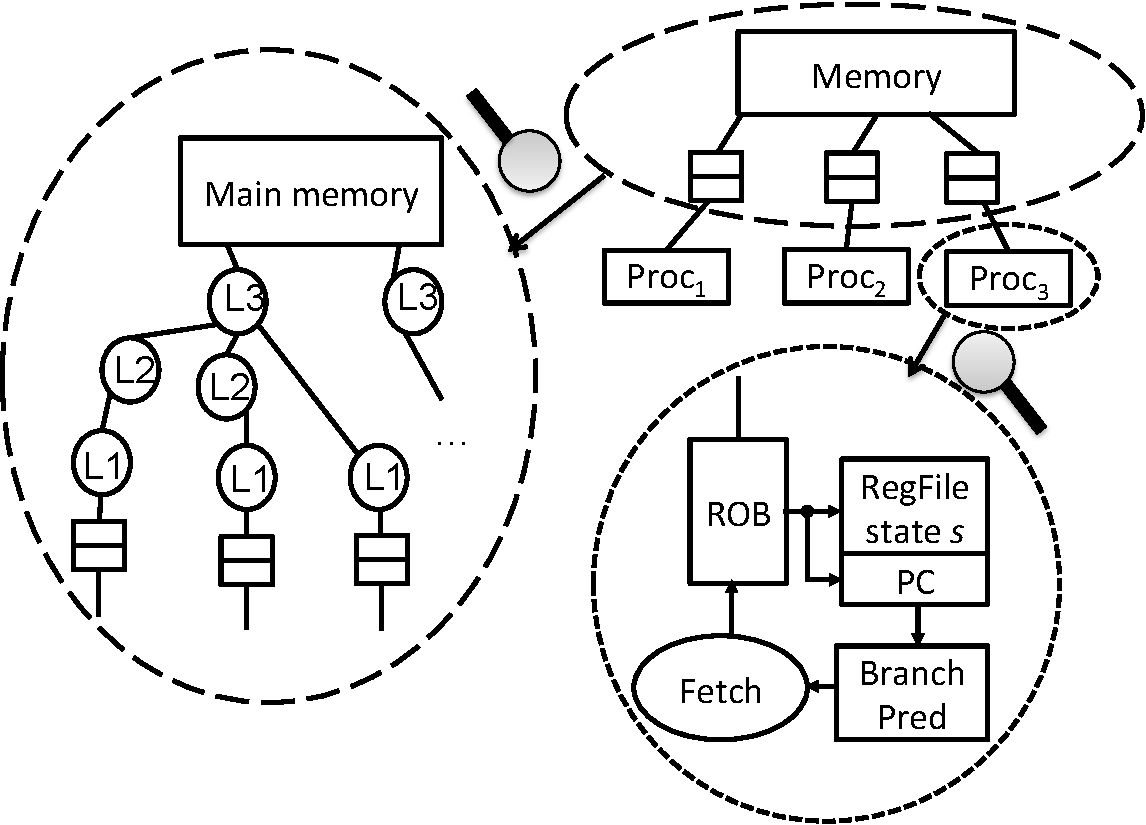
\includegraphics[scale=.43]{zoom}
%\caption{Overall system}
%\label{zoom}
%\end{figure}
%
%Figure \ref{zoom} sketches the sort of hardware system that we have verified.
%We show the top-level system design at top right, and we zoom in on boxes standing for the
%memory system and a single processor.
%
%Memory is composed of a \emph{hierarchy of caches}, where each cache node (labeled
%like ``L1,'' ``L2,'' etc.) communicates only with its neighbors in the graph.
%Each processor has a dedicated L1 cache, from which we do our best to satisfy
%all memory requests, to avoid the latency of a round-trip with main memory.
%With an L1 cache miss, we may still find a hit in a parent cache below the
%level of main memory, realizing a smaller but still significant speedup.
%We have verified a \emph{directory-based} protocol for coordinating an arbitrary
%tree of caches, where each node stores a conservative approximation of its
%children's states.
%
%A processor is decomposed into several components.  We have the normal
%architectural state, such as values of registers.  Our proofs are generic over
%\emph{a family of instruction set architectures}, with parameters for opcode sets and
%functions for executing opcodes and decoding them from memory.  Other key
%components are a \emph{branch predictor}, which guesses at the control-flow path
%that a processor will follow, to facilitate speculation; and a
%\emph{reorder buffer (ROB)}, which decides which instructions along that path to
%try executing ahead of schedule.  Our proofs apply to an arbitrary branch predictor,
%and they work for any reorder buffer satisfying a simple semantic condition.
%
%Figure~\ref{proofs} gives the overall proof structure that we employ to verify
%the system of Figure~\ref{zoom}. As we will explain later, $P_\text{so}$
%represents the speculative out-of-order processor, $M_c$ the cache memory,
%$M_m$ the simple memory, $P_\text{ref}$ a simple decoupled processor, and
%SC the simple reference model having multiple processors executing each
%instruction atomically thus implementing sequential consistency.  Notation
%$A^n$ is for $n$ copies of system $A$ running in parallel.
%$\sqsubseteq$ is a refinement operator, capturing a suitable notion of when
%one system implements another.  We go into more detail on the symbols from
%the figure in the rest of the paper.
%
%Our current framework establishes theorems of the form ``if system $A$ has a run
%with some particular observable behavior, then system $B$ also has a run with
%the same behavior.''  In this sense, we say that $A$ correctly implements $B$.
%Other important properties, such as \emph{deadlock freedom} for $A$ (which
%might get stuck without producing any useful behavior), we leave for future
%work.
%
%\begin{figure}
%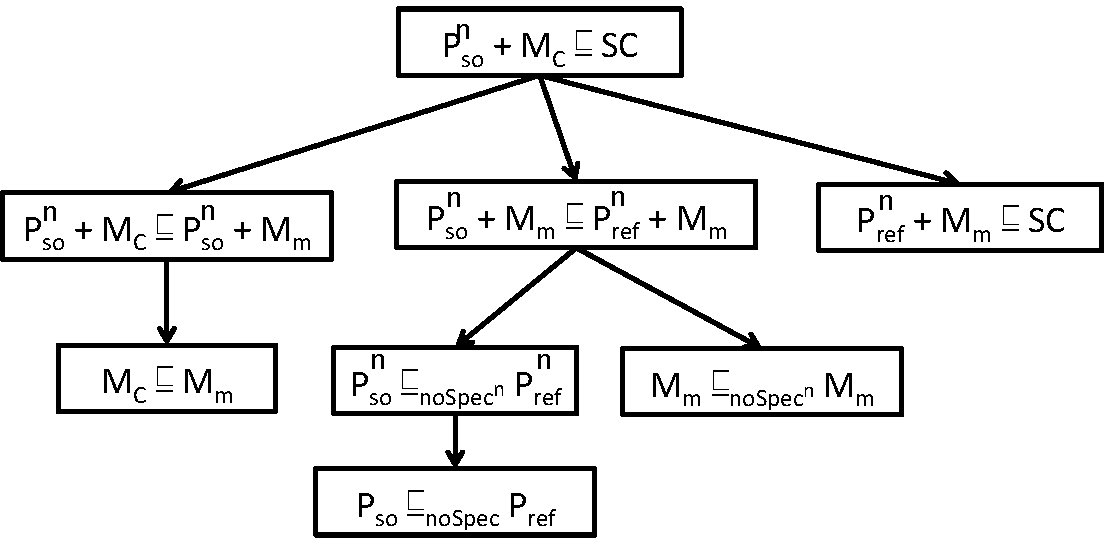
\includegraphics[scale=.45]{proofs}
%\caption{Overall proof structure}
%\label{proofs}
%\end{figure}


%% Modularity has long been understood as a key property for effective design and
%% verification of complex systems, \eg\ distributed memory systems. For the
%% designer, it allows a separation of concerns increasing robustness by allowing
%% the behavior encapsulated by a modular boundary to be realized by multiple
%% implementation any of which may be safely dropped into the system. It also
%% allows a greater measure of parallelization of design improving development
%% time. Similarly verification is simplified as modular interface agreements
%% provide a set of natural lemmas to verify. This leads us towards a
%% decomposition of the whole system verification task into smaller more
%% manageable chunks.

%% Given its complexity, it is a practical necessity for distributed shared memory
%% systems to be built a strong idea of modularity. The standard modularization
%% (see Figure~\ref{fig:highleveldsm}) separates the ISA-level processors nodes
%% which are responsible for executing threads of computation, and a unified
%% shared memory subsystem which is responsible for ensuring that memory requests
%% it receives are handled correctly, \ie{} in line with the memory model which
%% dictates which store values a load may observe in the system. These processors
%% may then be refined for performance, while the monolithic memory module is
%% improved by introducing layers of caching and a coherence protocol to guarantee
%% memory consistency.

%% This high-level approaches works reasonably well for implementation; separate
%% design groups tackle can each task in isolation. However, when we consider
%% verification, the modularity enforced during the implementation has little
%% benefit and in practice we must resort to full system verification. The core of
%% this problem lies in the fact that the simple high-level decomposition of
%% memory and processors does not fully take into account the space of speculation
%% techniques used in the processor.

%% All practical processor instruction set architectures (ISAs) are fairly
%% sequential; the result of executing an instruction may affect which next
%% instruction is executed. As a result for performance some sort of prediction is
%% used to allow instructions to be speculatively started and executed before the
%% previous instructions have completed and the values need to execute are known.
%% Additional bookkeeping is used to determine when our guess is wrong and
%% false-path instructions are undone leaving no affect on the architectural
%% state. As precise exception handling is a requirement these speculative
%% instructions are committed, \ie{} expose their effects of execution to the
%% whole system, in sequence.

%% Though most forms of speculation (\eg{} branch prediction, instruction prefetch
%% from pipelining, value prediction) are often considered as being orthogonal to
%% memory issues, speculation changes the sequence of memory requests the
%% processor sends to the memory. This may be merely handling requests out of
%% order, \eg{} issuing a load request before a logically earlier one has issued
%% (a common occurrence due to data dependencies in out-of-order processors). We
%% may also allow incorrect memory operations to be issued, \eg{} executing a load
%% from a false path. It is worth noting that while such load operations are
%% possible to speculate, we cannot speculatively issues store operations to the
%% memory as they become exposed to the whole system and speculation mechanisms
%% are isolated to a single processor. As a consequence of this, our memory does
%% not know what order requests it is sent should happen. Thus the memory in
%% isolation cannot directly realize the memory model and in actually implements a
%% much weaker model leaving the full enforcement of the memory model to the
%% processor which can enforce this by restricting when it issues requests. 

%% The goal of this work is to introduce an interface enabling true modular
%% implementation and verification of shared memory systems. That is, we should be
%% able to describe a modular decomposition where we may correct replace either
%% the processor nodes, the memory with locally verified alternatives without
%% changing the correctness of our whole system proof of correctness or
%% restricting our ability to describe shared memory systems. As part of this we
%% will describe the processor interface in a way which allows the full range of speculation 

%% We do so by showing the construction and initial refinements of a sequentially
%% consistent shared memory system. We formally defining a minimal cache coherent
%% speculation-friendly memory interface (\emph{Store Atomicity}), and use this as
%% the interface for our memory subsystem. Using this we specify the notion of
%% correct for a processor and prove that our system is correct assuming the
%% correct implementation of these two objects.  We then construct both a naive
%% reference processor and memory subsystem and provide proofs of correctness in
%% Coq. We then refine both components into more realistic implementations
%% including taking our memory subsystem to hardware-level description of a
%% arbitrary-level hierarchical cache coherence implementation and verify these
%% module. We show that the cross products of possible implementations are correct
%% and their proof automatically from the modularly.

%%  LocalWords:  Modularity modularity



